\documentclass{article}
\usepackage{graphicx}
\usepackage{caption}
\captionsetup[figure]{labelformat=empty}
\usepackage[margin=3cm]{geometry}

\begin{document}

\centering

\begin{figure}	
	\caption{FIGURE 1} 
		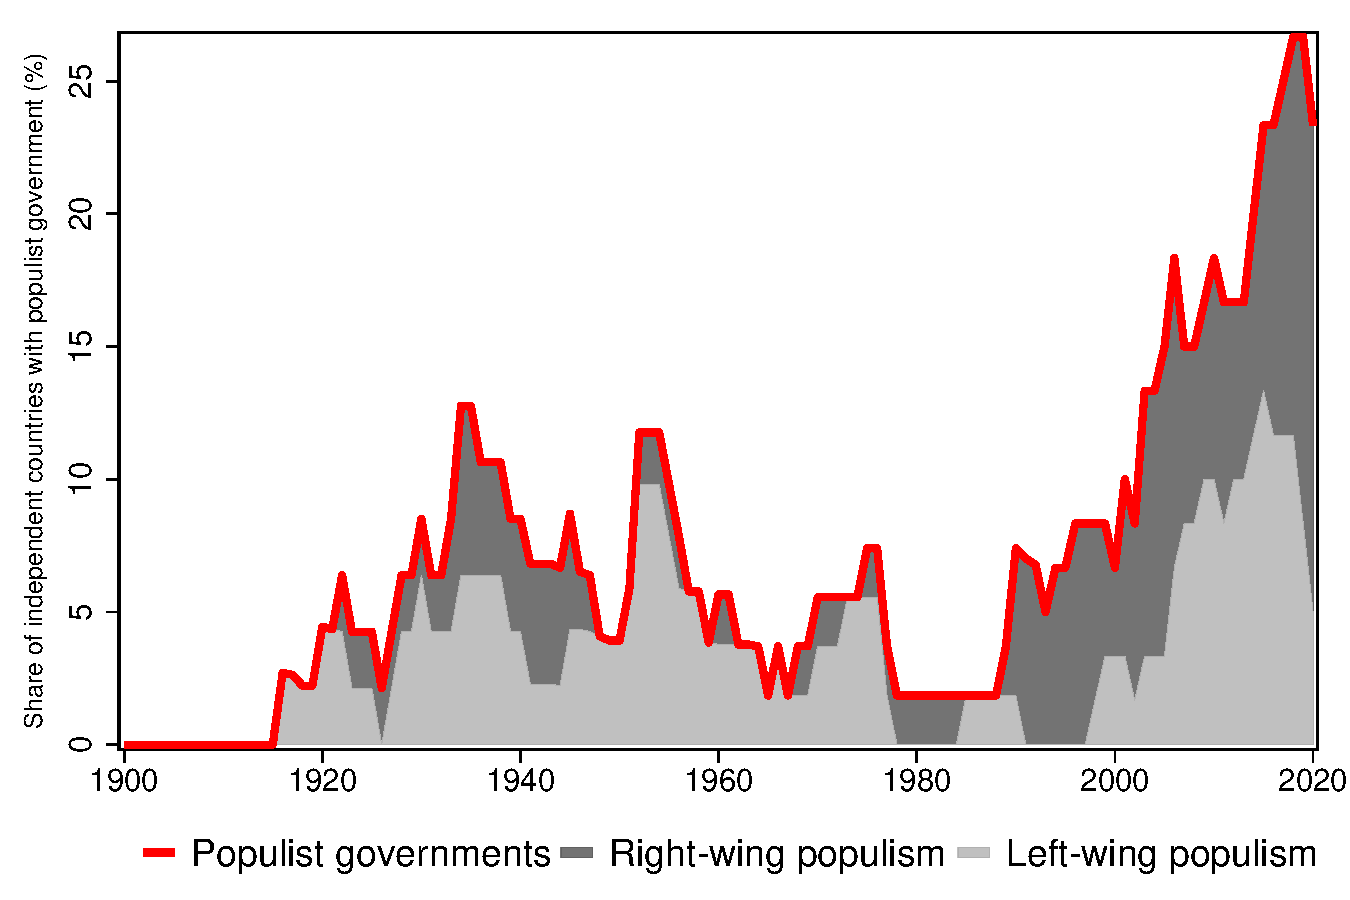
\includegraphics[scale=0.6]{Figure1}\centering	
\end{figure}

\clearpage

\begin{figure}	
	\caption{FIGURE 2} 
		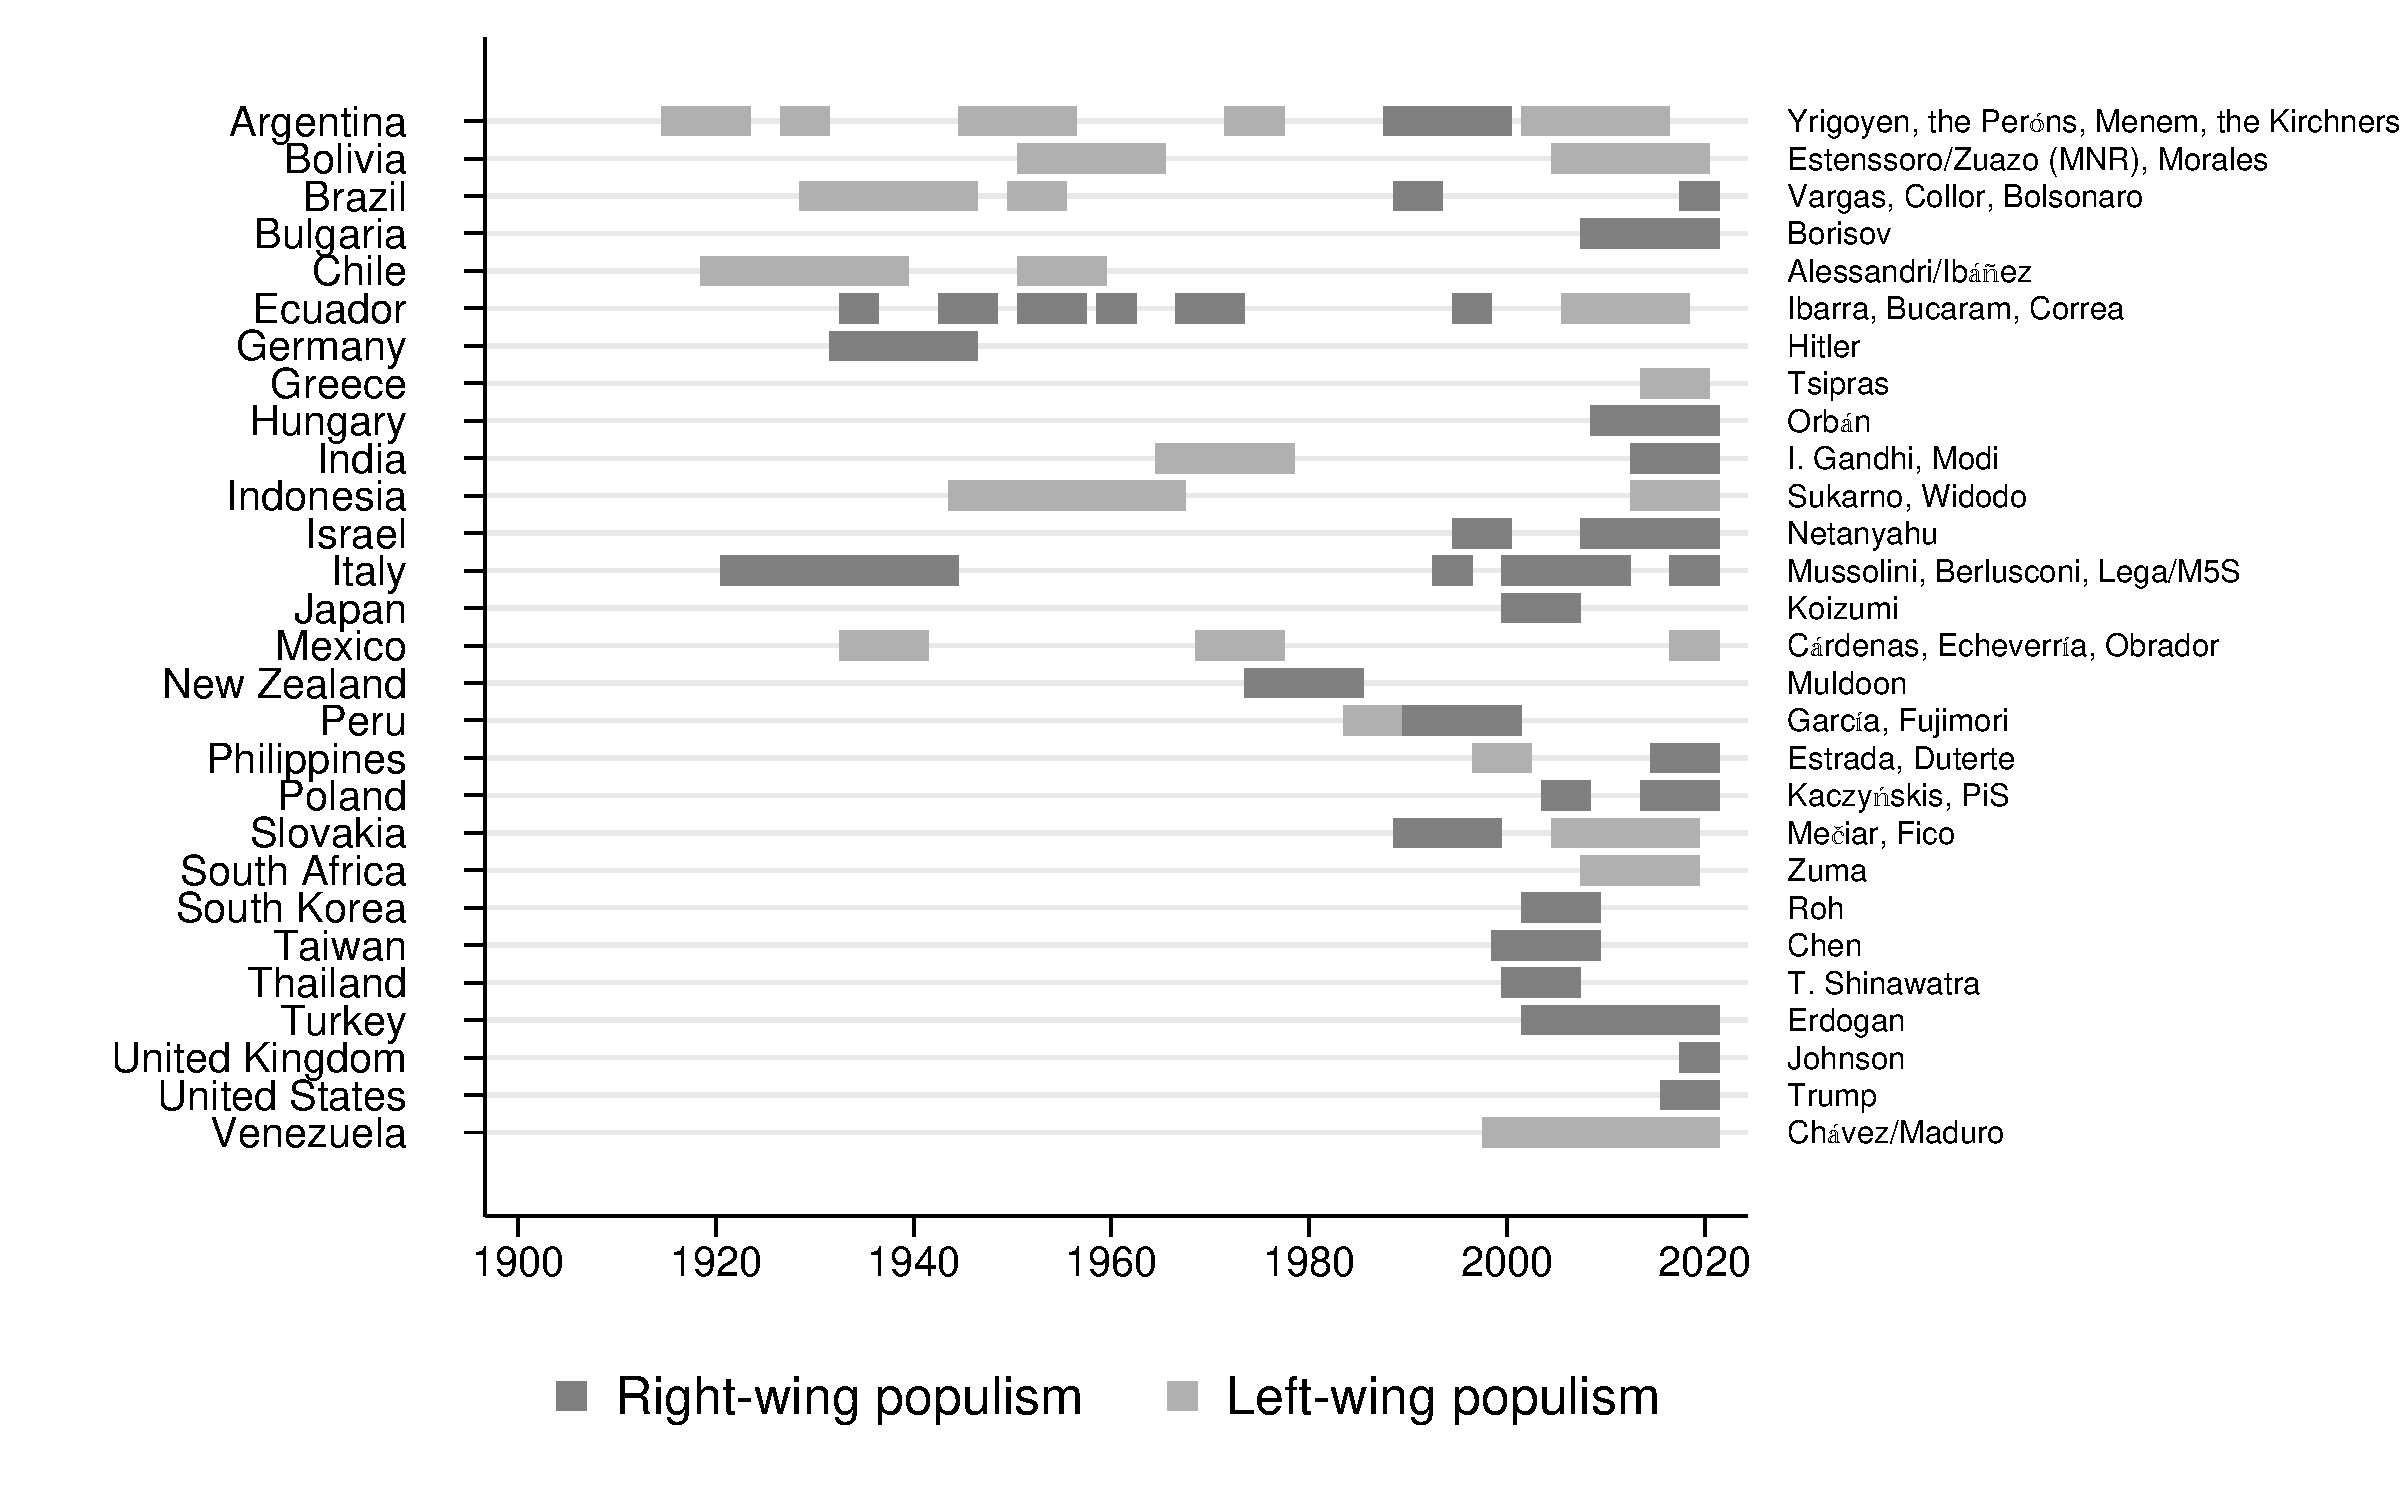
\includegraphics[scale=0.35]{Figure2}\centering	
\end{figure}

\clearpage

\begin{figure}	
	\caption{FIGURE 3} 
		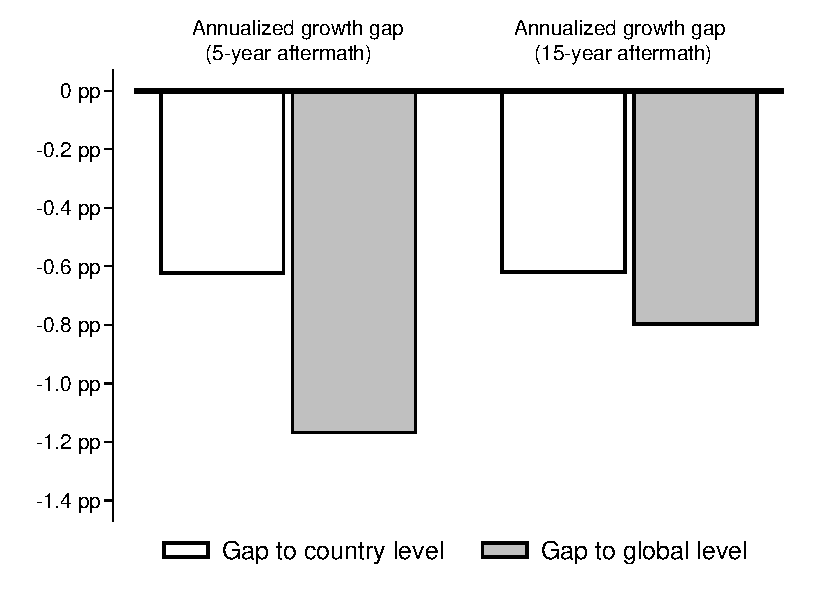
\includegraphics[scale=0.7]{Figure3}\centering	
\end{figure}

\clearpage

\begin{figure}	
	\caption{FIGURE 4} 
		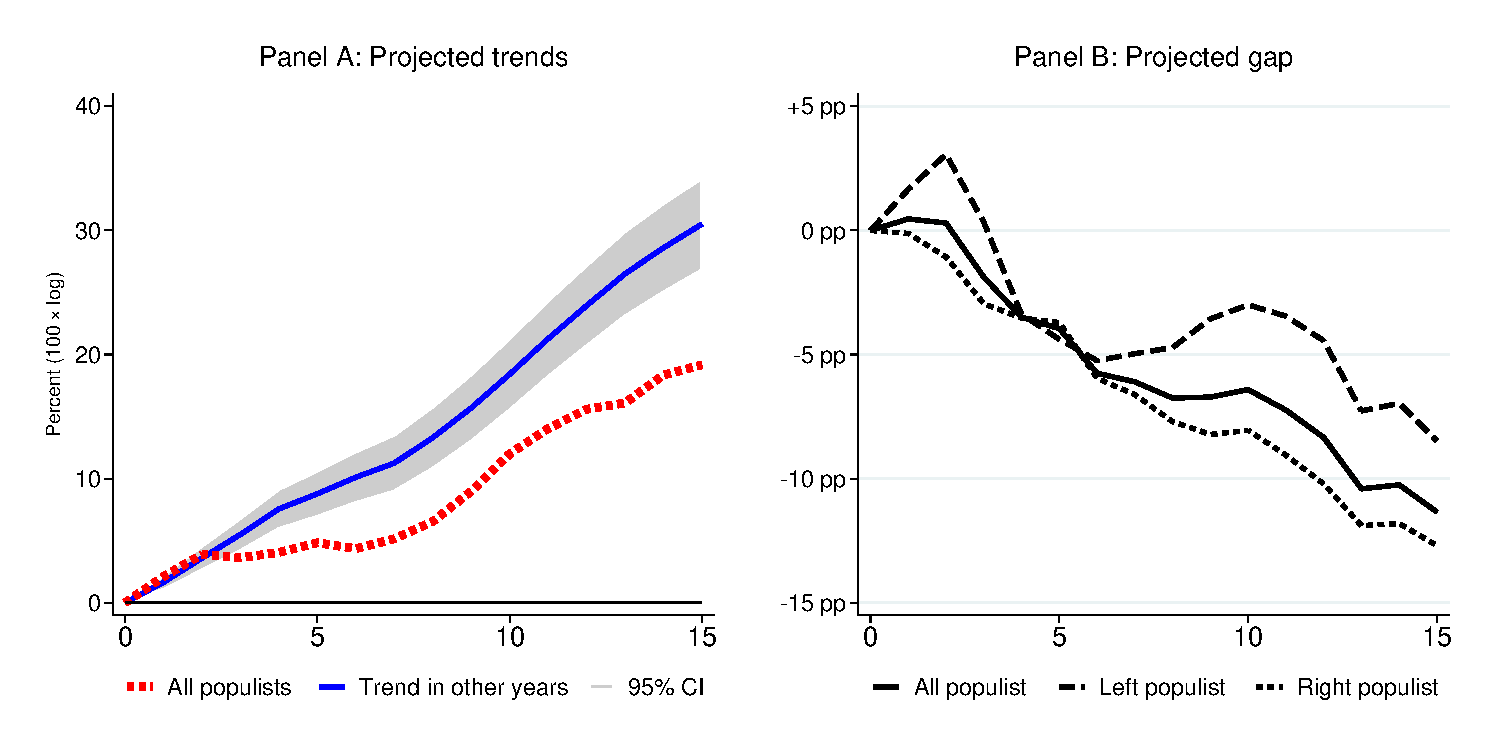
\includegraphics[scale=0.6]{Figure4}\centering	
\end{figure}

\clearpage

\begin{figure}	
	\caption{FIGURE 5} 
		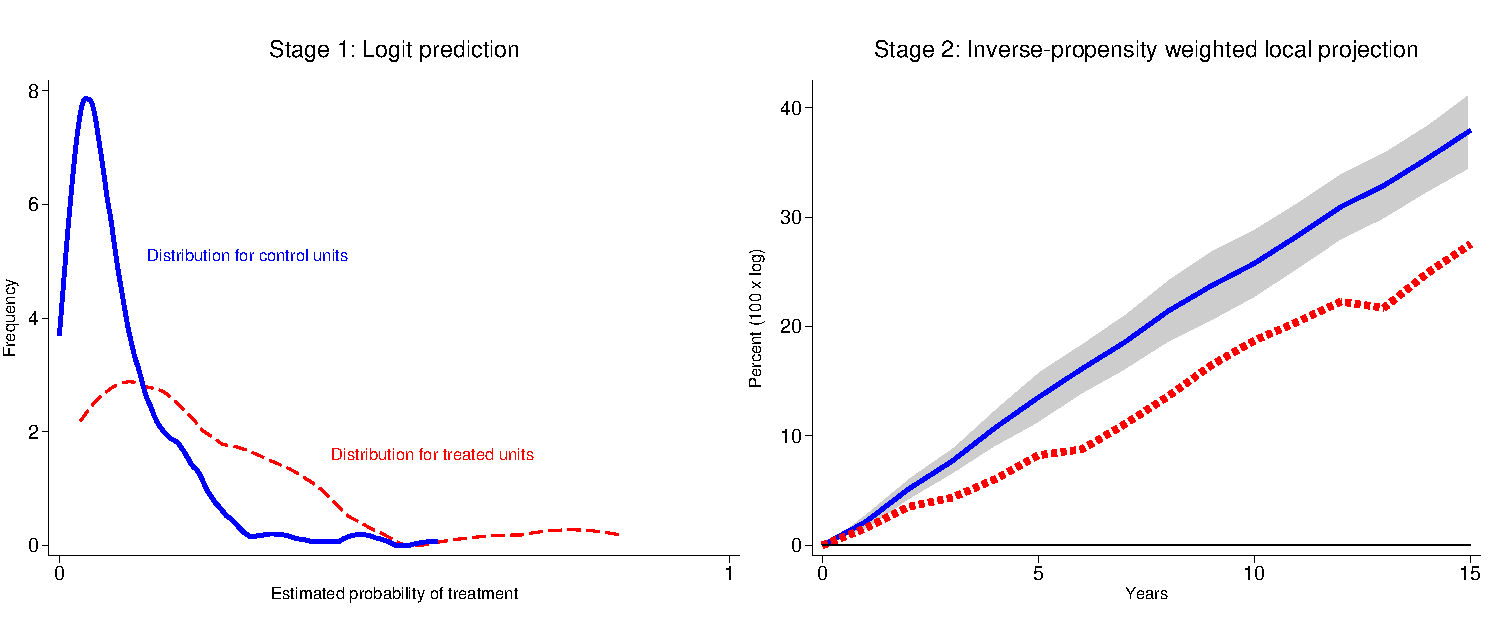
\includegraphics[scale=0.6]{Figure5}\centering	
\end{figure}

\clearpage

\begin{figure}	
	\caption{FIGURE 6} 
		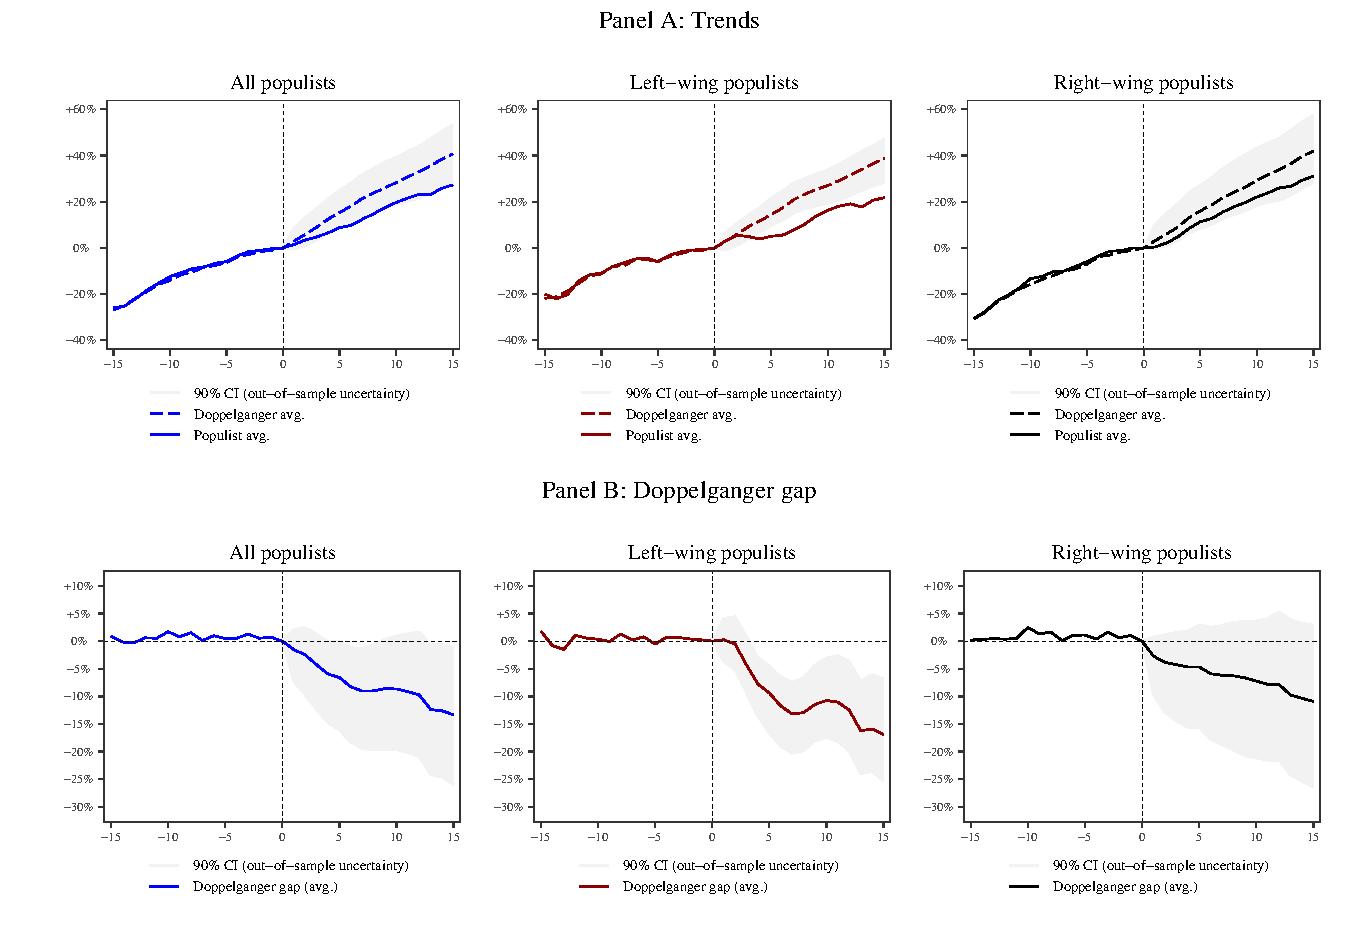
\includegraphics[scale=0.6]{Figure6}\centering	
\end{figure}

\clearpage

\begin{figure}	
	\caption{FIGURE 7} 
		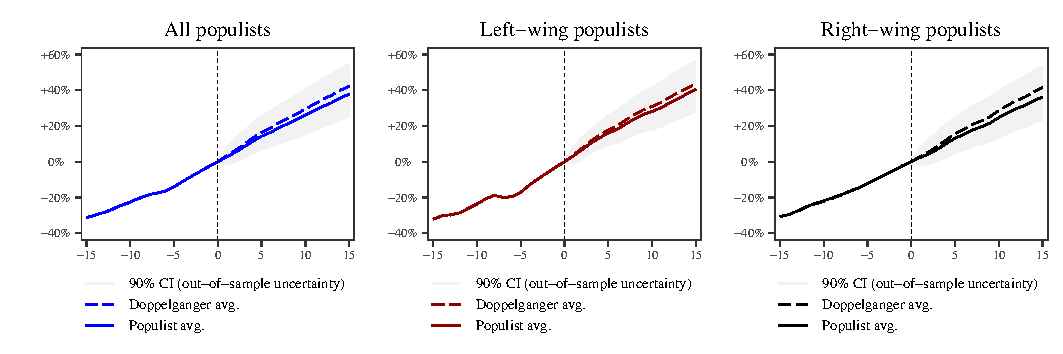
\includegraphics[scale=0.8]{Figure7}\centering	
\end{figure}

\clearpage

\begin{figure}	
	\caption{FIGURE 8} 
		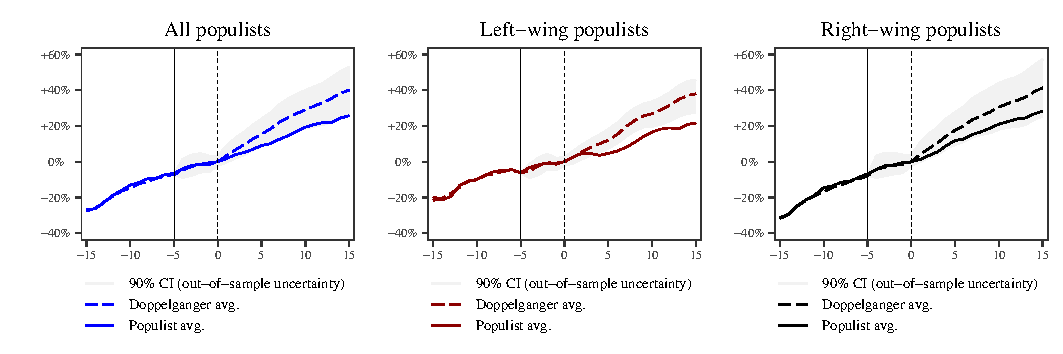
\includegraphics[scale=0.8]{Figure8}\centering	
\end{figure}

\clearpage

\begin{figure}	
	\caption{FIGURE 9} 
		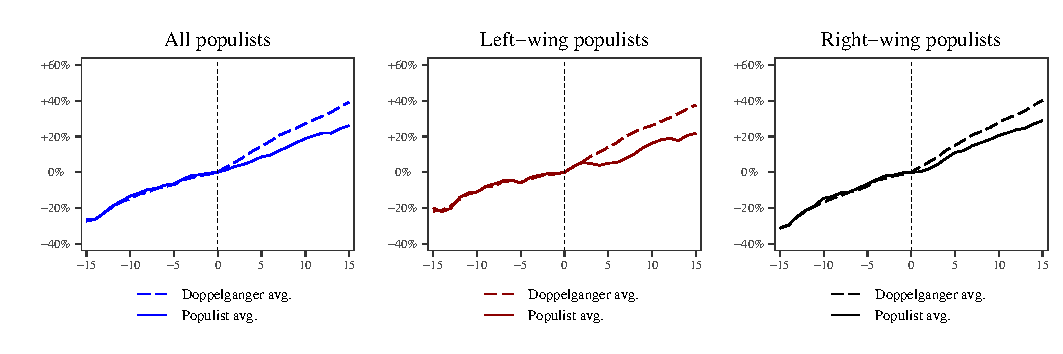
\includegraphics[scale=0.8]{Figure9}\centering	
\end{figure}

\clearpage

\begin{figure}	
	\caption{FIGURE 10} 
		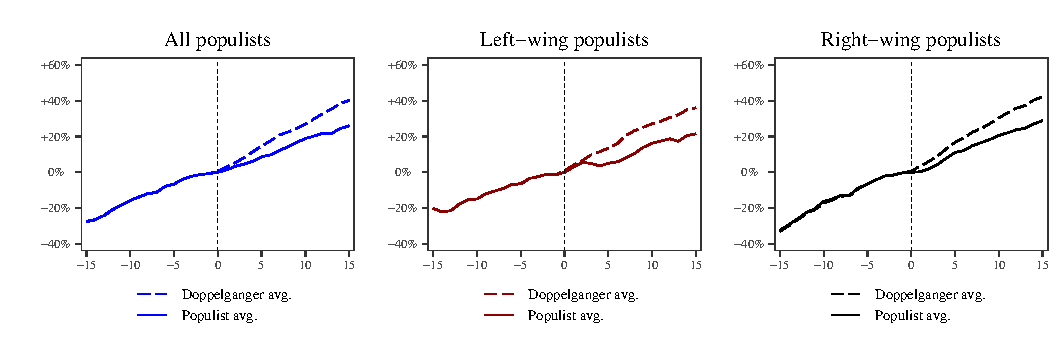
\includegraphics[scale=0.8]{Figure10}\centering	
\end{figure}

\clearpage

\begin{figure}	
	\caption{FIGURE 11} 
		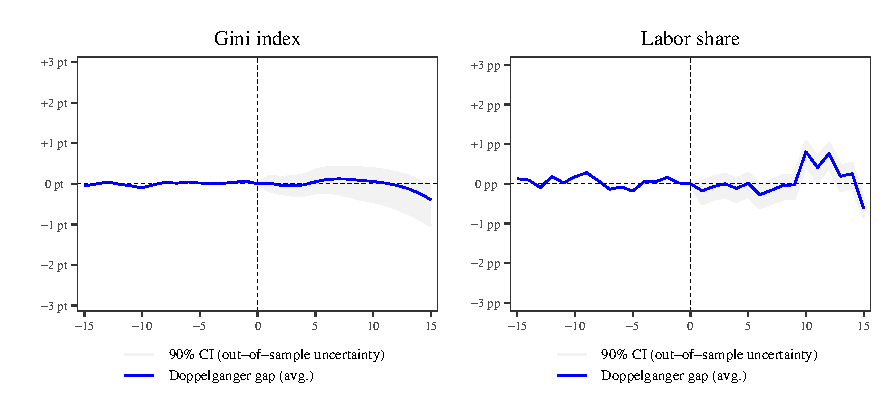
\includegraphics[scale=0.8]{Figure11}\centering	
\end{figure}

\clearpage

\begin{figure}	
	\caption{FIGURE 12} 
		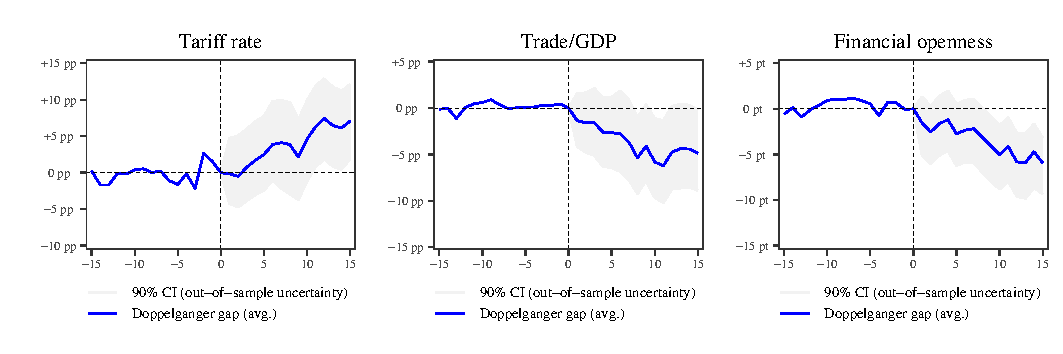
\includegraphics[scale=0.8]{Figure12}\centering	
\end{figure}

\clearpage

\begin{figure}	
	\caption{FIGURE 13} 
		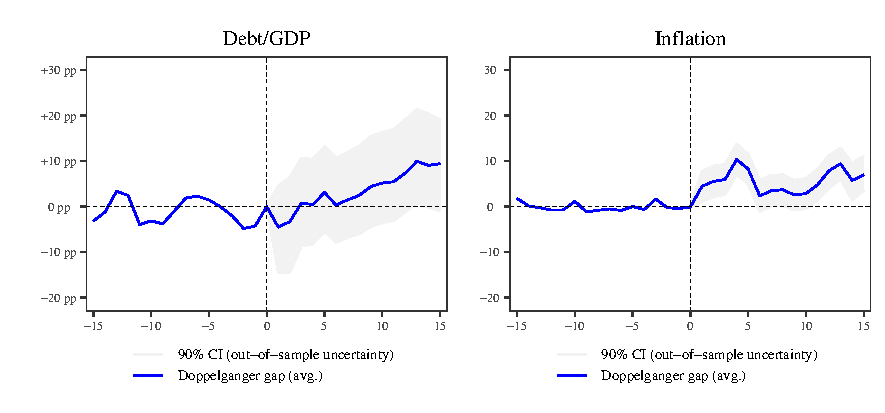
\includegraphics[scale=0.8]{Figure13}\centering	
\end{figure}

\clearpage

\begin{figure}	
	\caption{FIGURE 14} 
		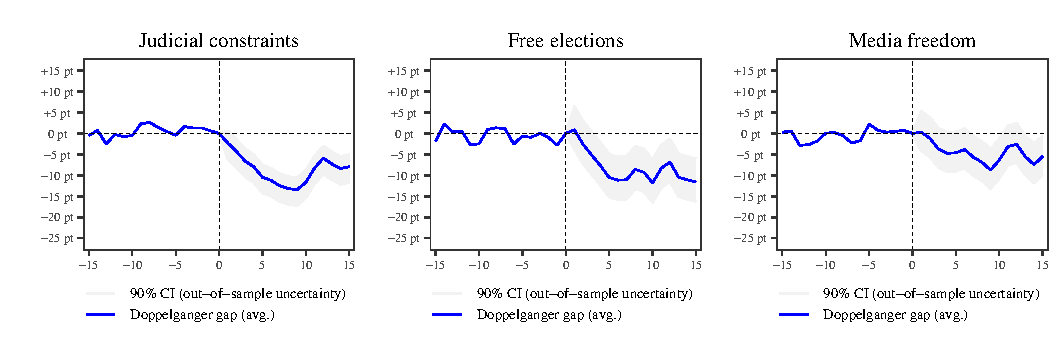
\includegraphics[scale=0.8]{Figure14}\centering	
\end{figure}

\clearpage

\begin{figure}	
	\caption{FIGURE A1} 
		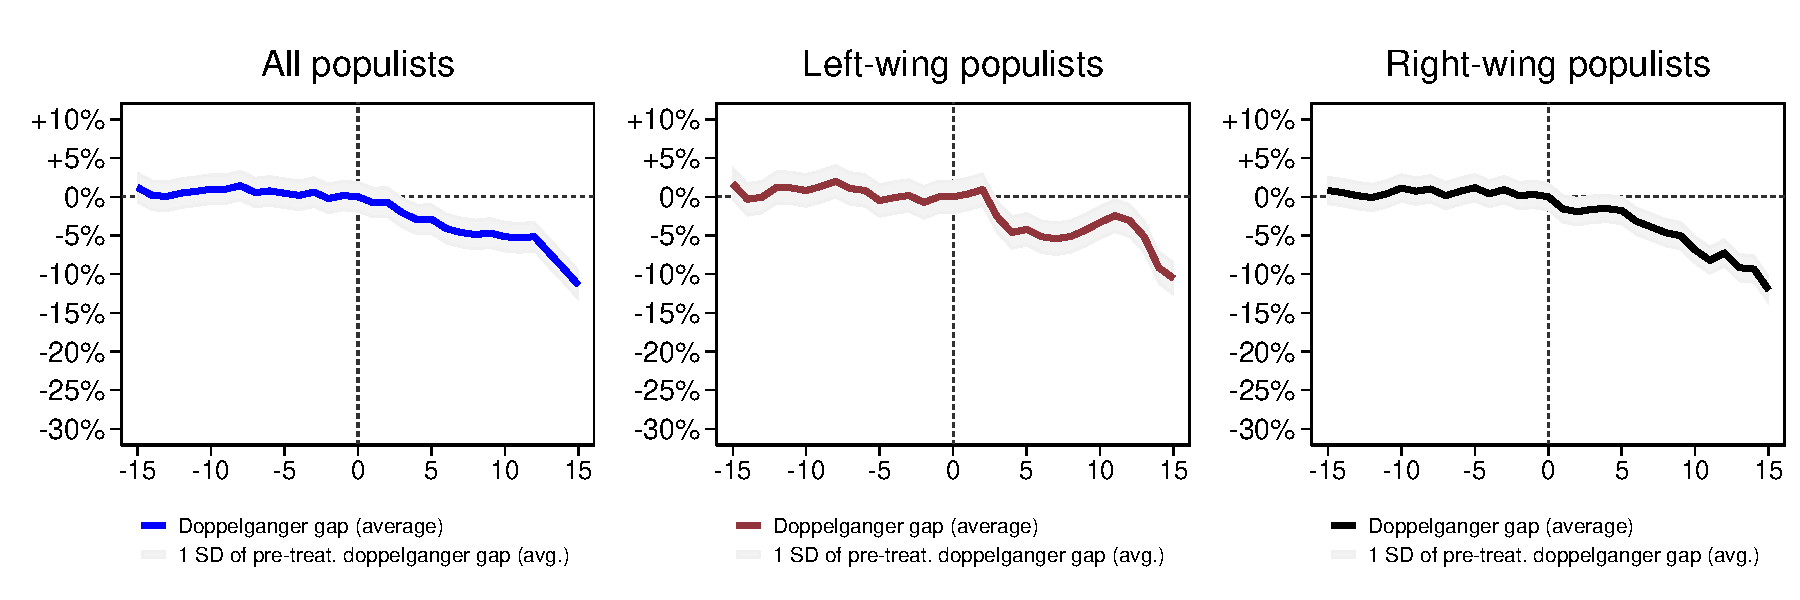
\includegraphics[scale=0.5]{FigureA1}\centering	
\end{figure}

\clearpage

\begin{figure}	
	\caption{FIGURE A2} 
		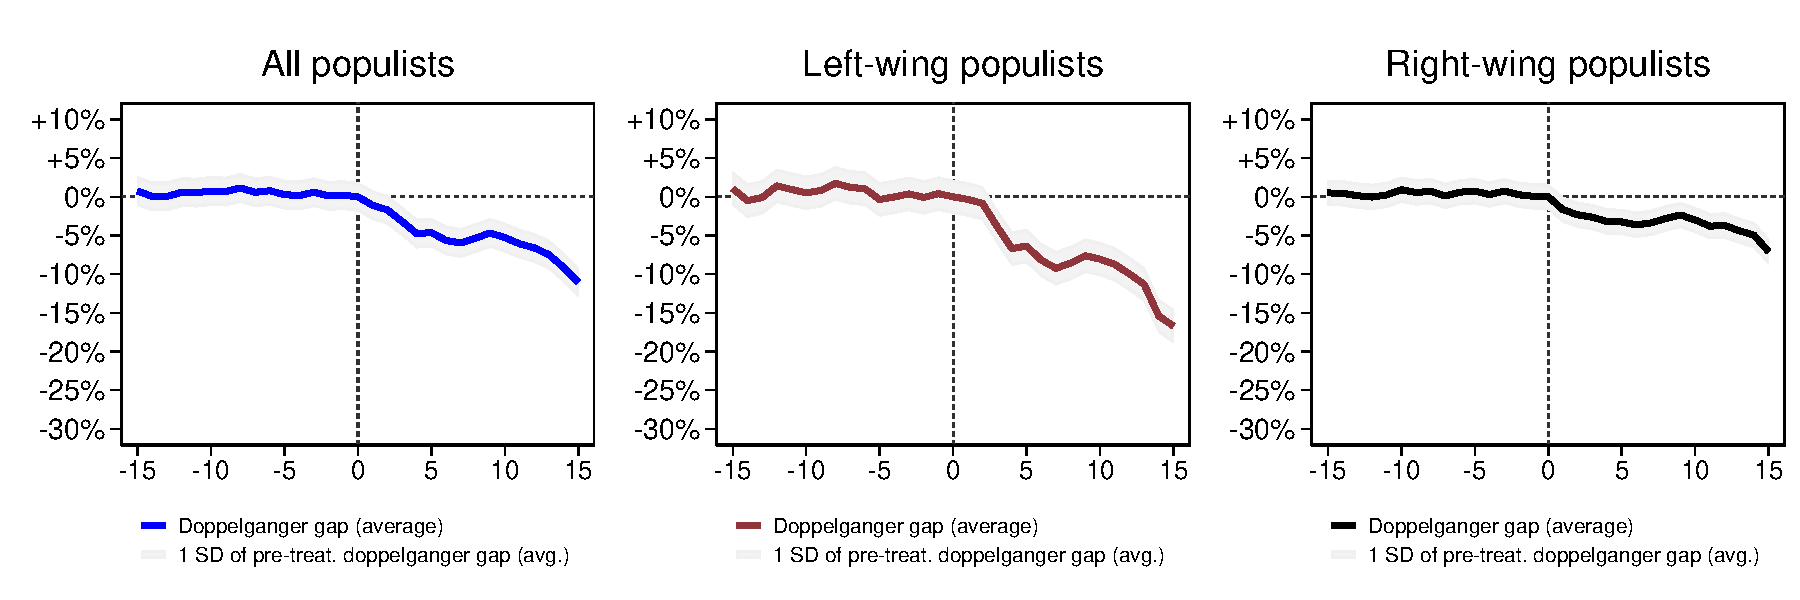
\includegraphics[scale=0.5]{FigureA2}\centering	
\end{figure}

\clearpage

\begin{figure}	
	\caption{FIGURE A3} 
		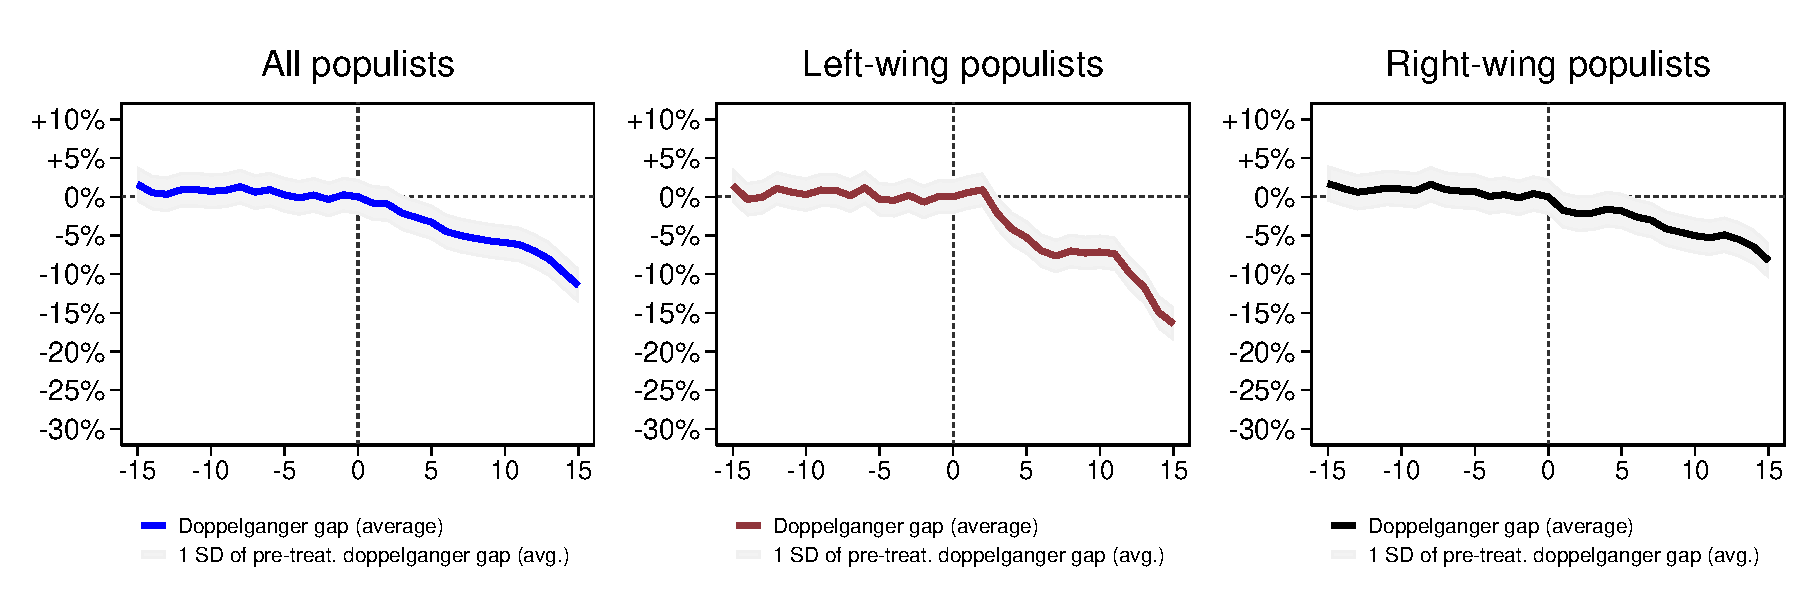
\includegraphics[scale=0.5]{FigureA3}\centering	
\end{figure}

\clearpage

\begin{figure}	
	\caption{FIGURE B1} 
		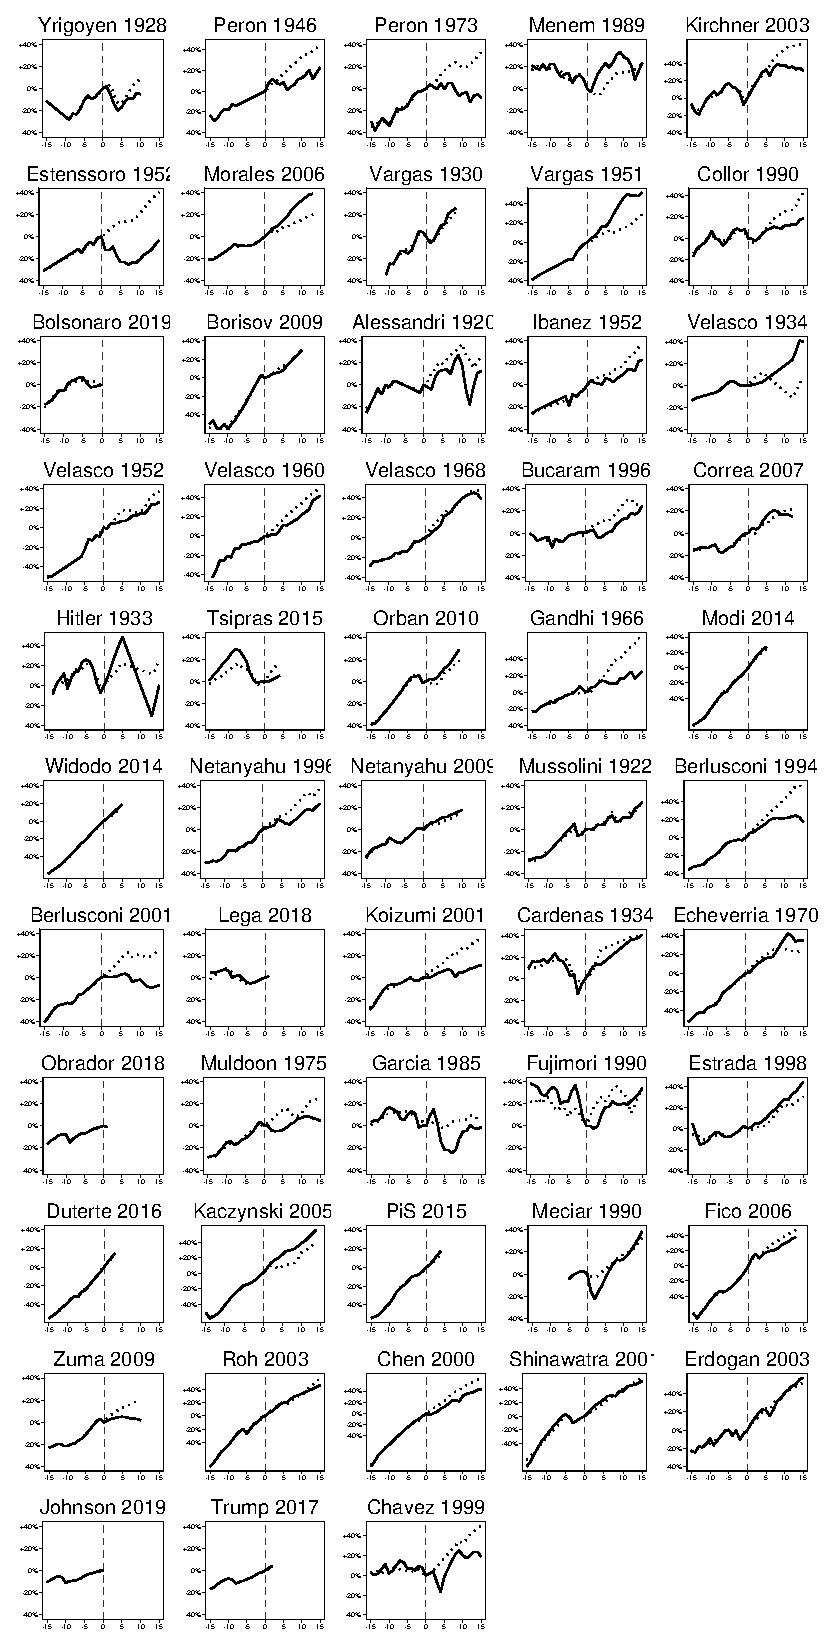
\includegraphics[scale=0.7]{FigureB1}\centering	
\end{figure}

\begin{figure}	
	\caption{FIGURE B2} 
		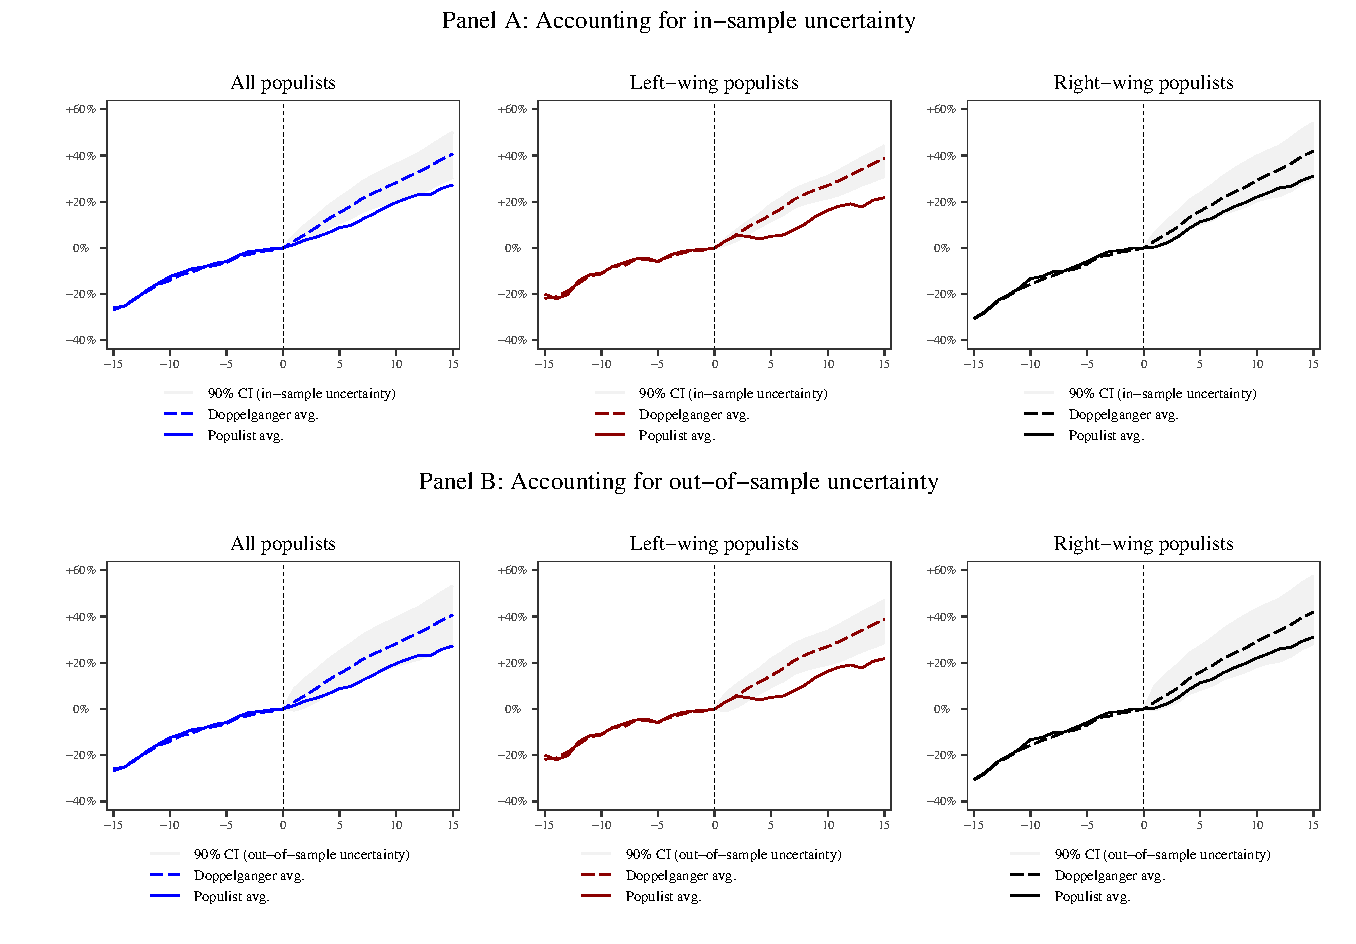
\includegraphics[scale=0.6]{FigureB2}\centering	
\end{figure}

\clearpage

\begin{figure}	
	\caption{FIGURE B3} 
		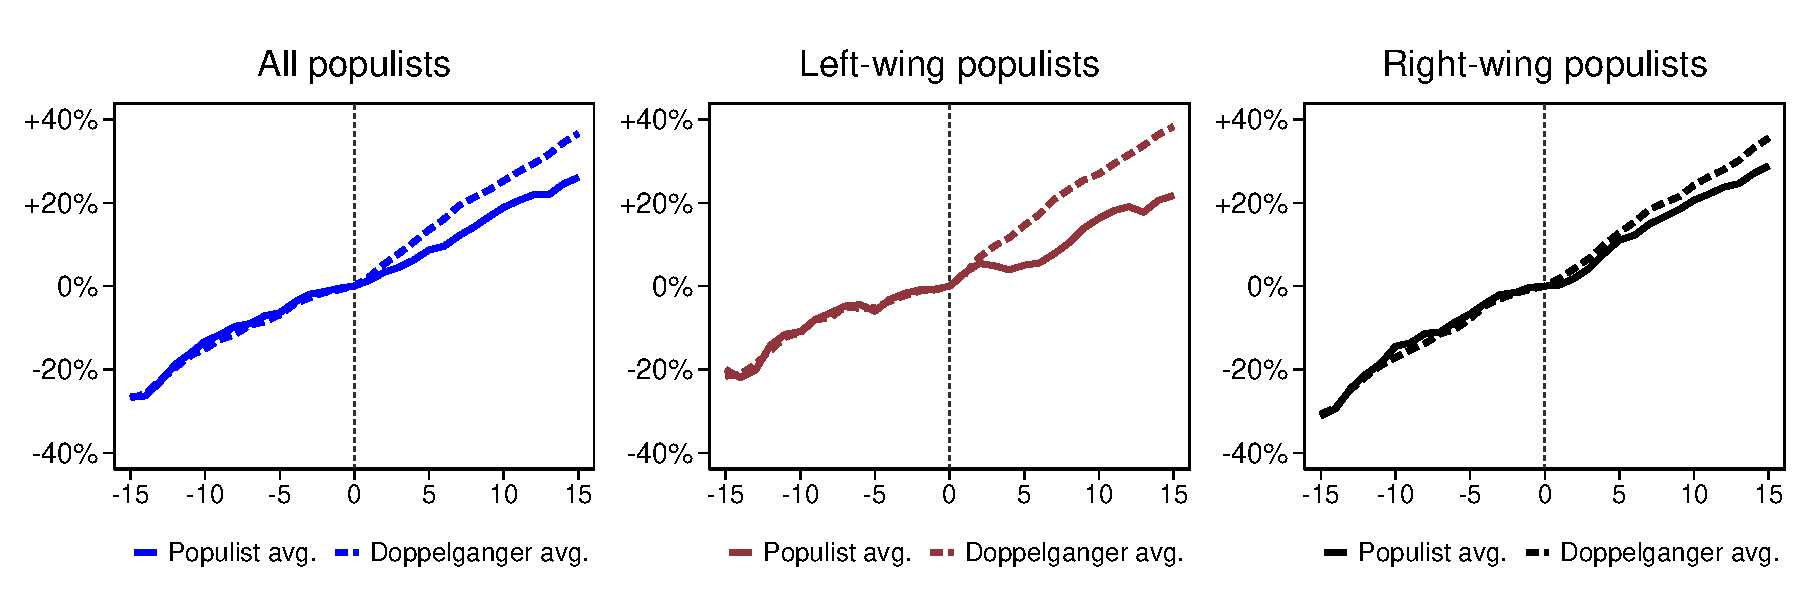
\includegraphics[scale=0.5]{FigureB3}\centering	
\end{figure}

\clearpage

\begin{figure}	
	\caption{FIGURE B4} 
		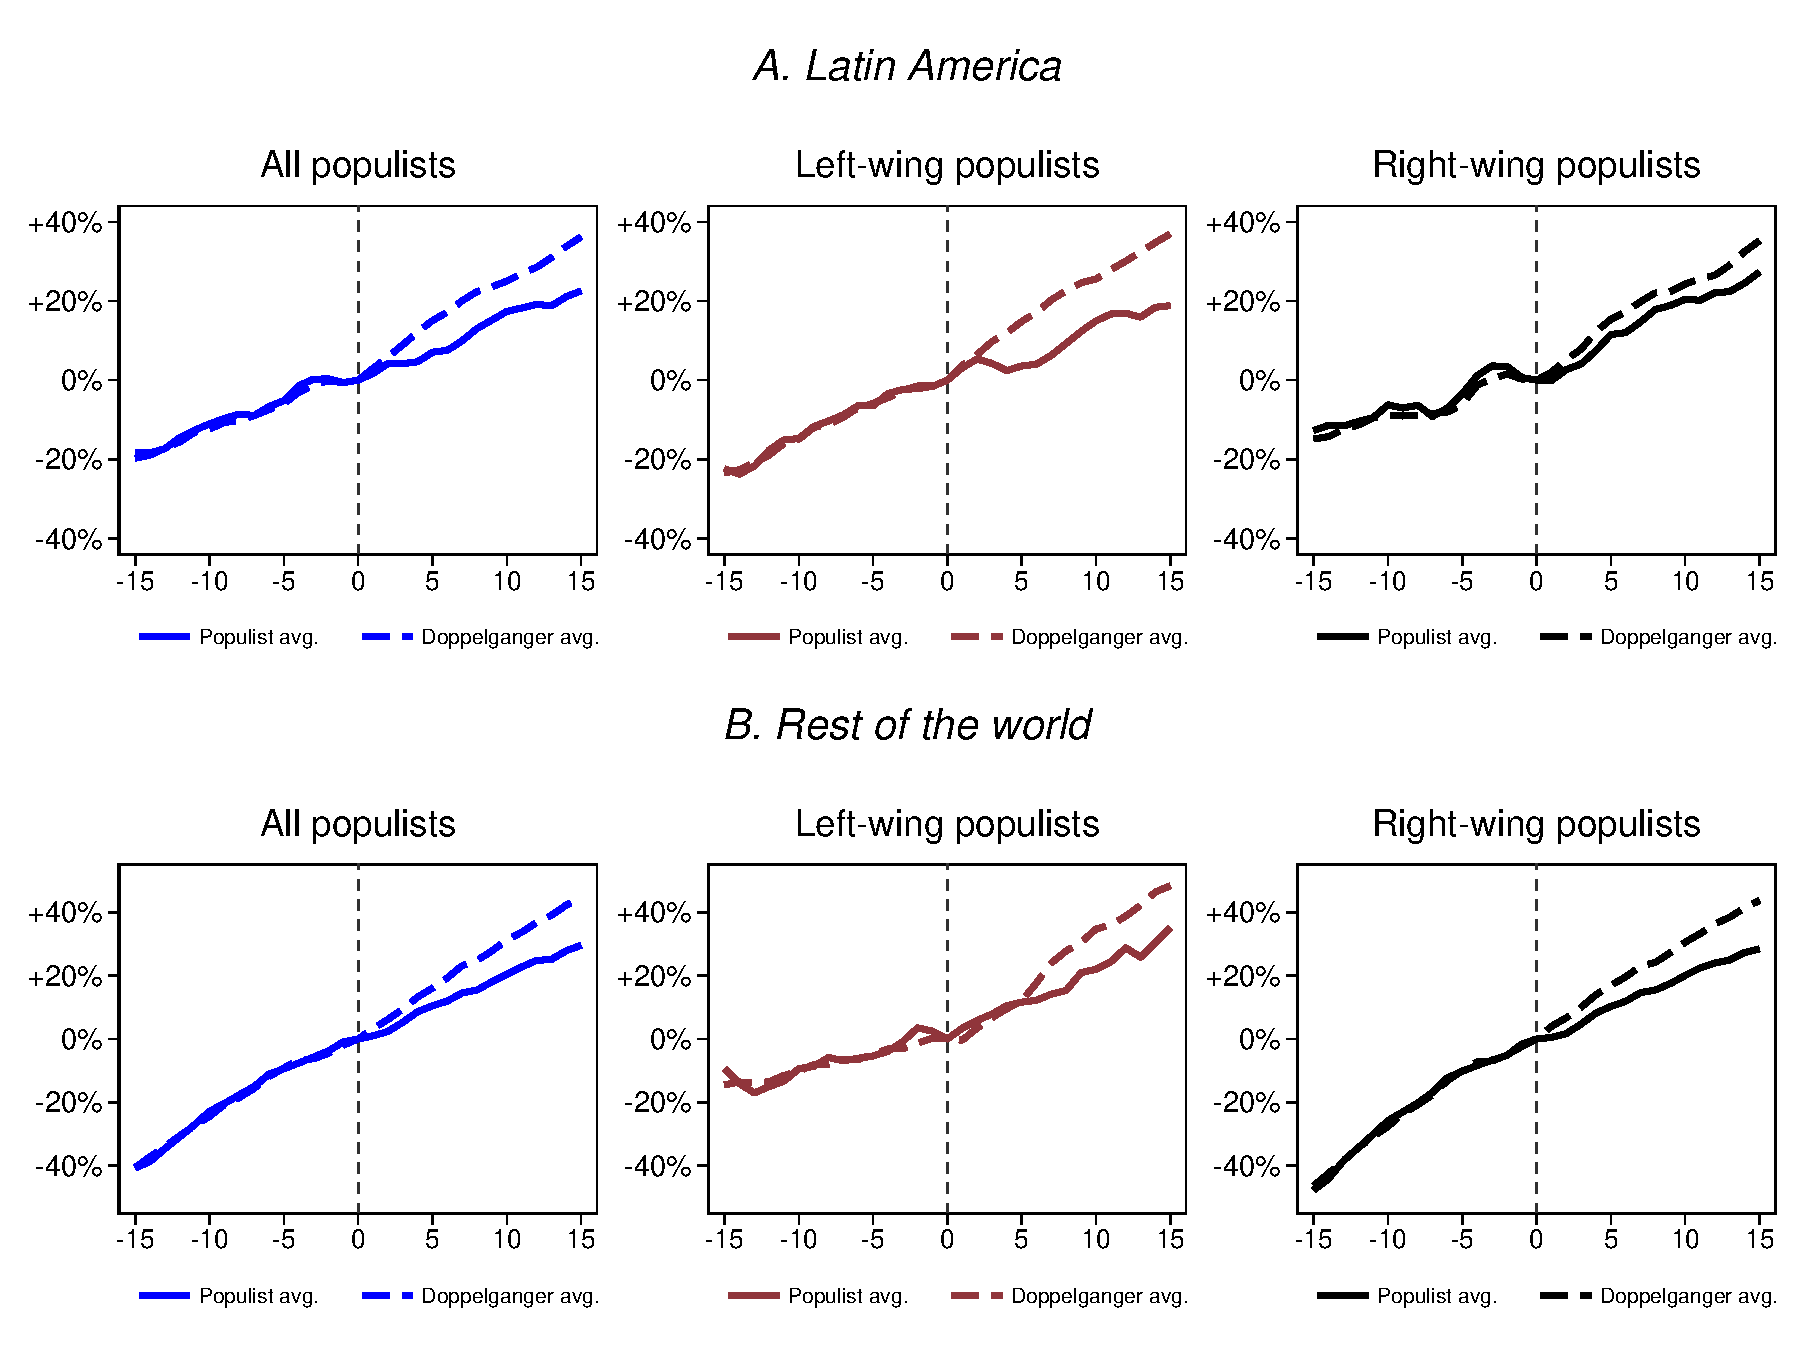
\includegraphics[scale=0.5]{FigureB4}\centering	
\end{figure}

\clearpage

\begin{figure}	
	\caption{FIGURE B5} 
		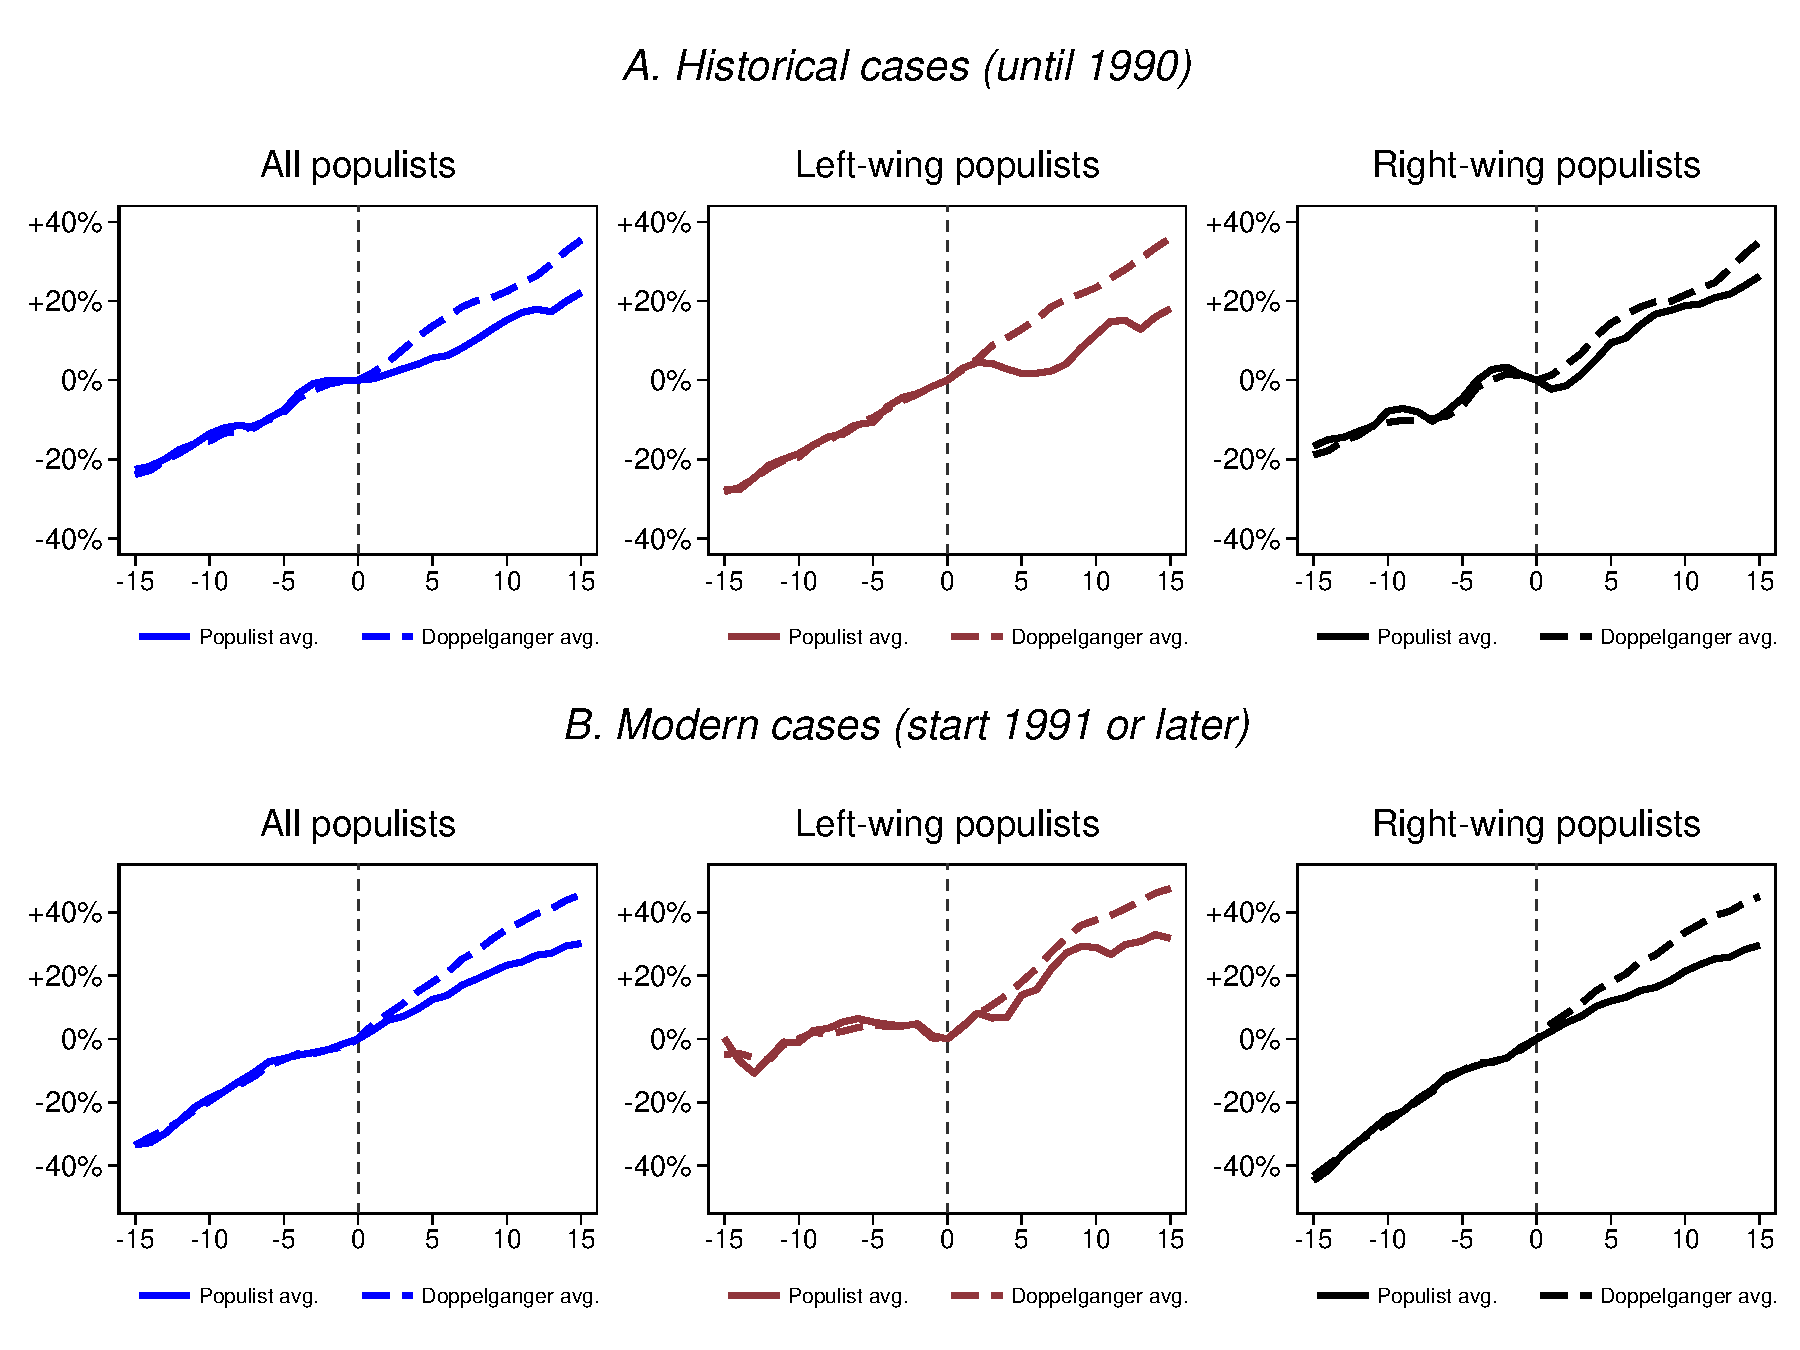
\includegraphics[scale=0.5]{FigureB5}\centering	
\end{figure}

\clearpage

\begin{figure}	
	\caption{FIGURE B6} 
		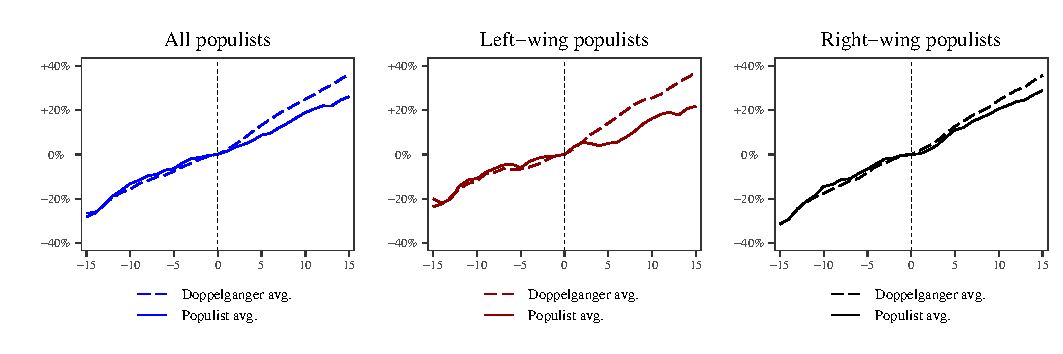
\includegraphics[scale=0.8]{FigureB6}\centering	
\end{figure}

\clearpage

\begin{figure}	
	\caption{FIGURE B7} 
		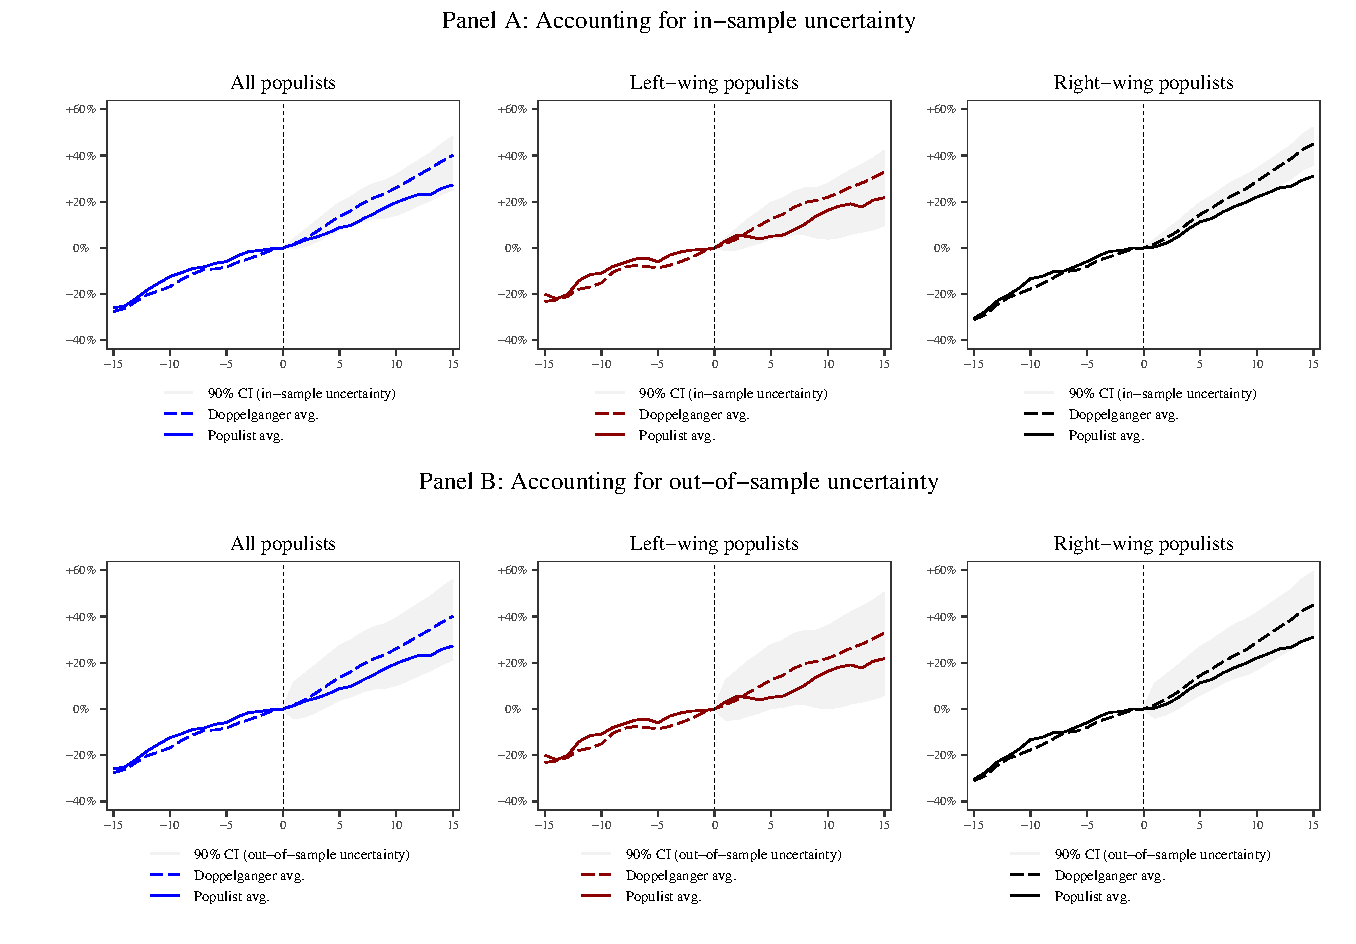
\includegraphics[scale=0.6]{FigureB7}\centering	
\end{figure}

\clearpage

\begin{figure}	
	\caption{FIGURE B8} 
		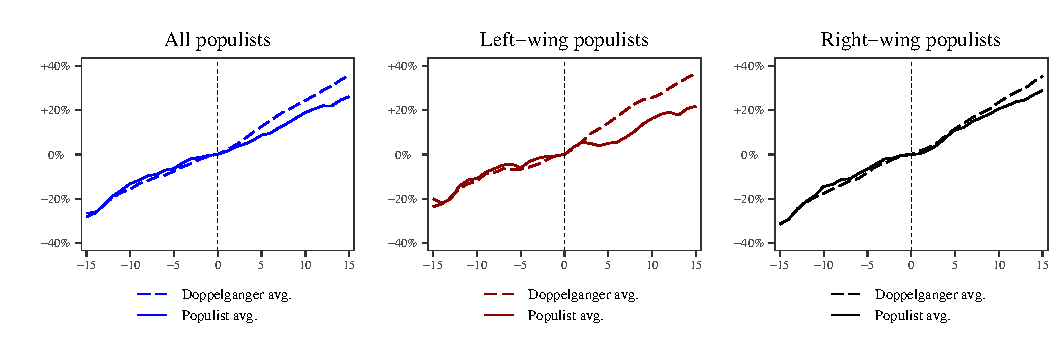
\includegraphics[scale=0.8]{FigureB8}\centering	
\end{figure}

\clearpage

\begin{figure}	
	\caption{FIGURE B9} 
		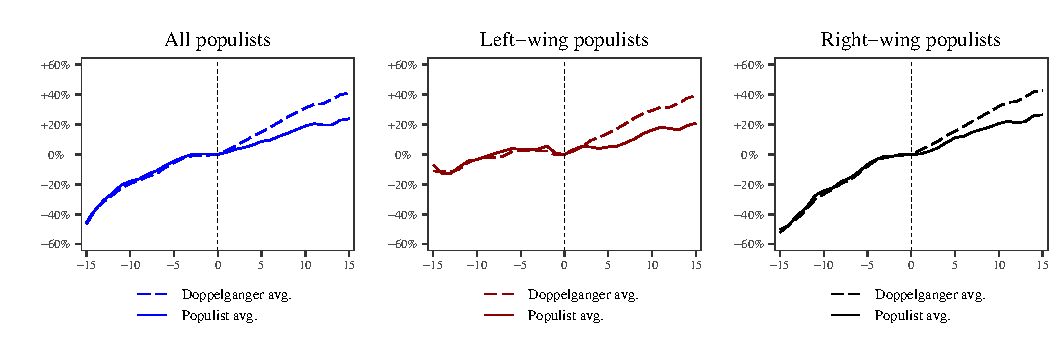
\includegraphics[scale=0.8]{FigureB9}\centering	
\end{figure}

\clearpage

\begin{figure}	
	\caption{FIGURE C1} 
		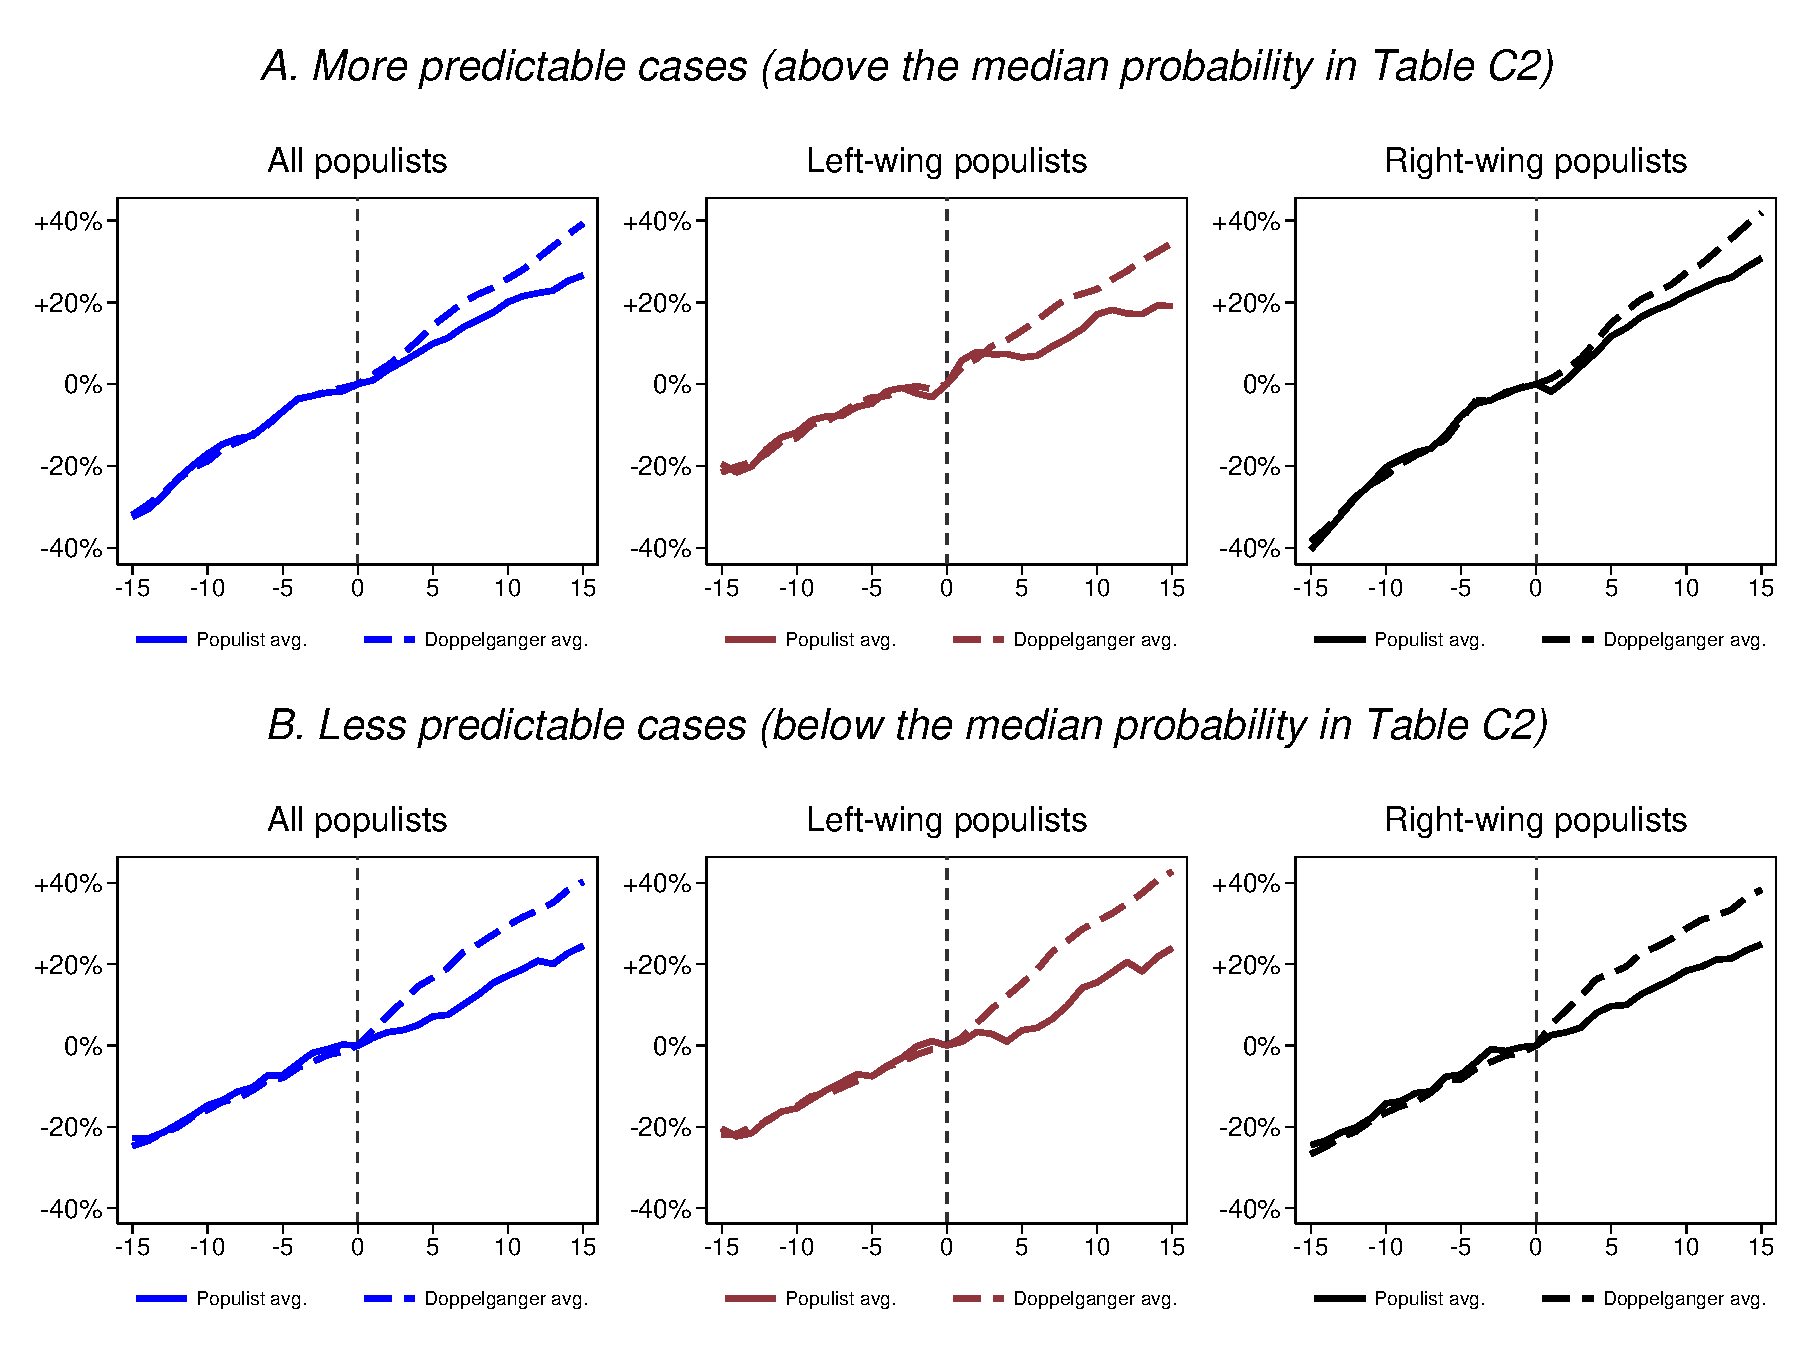
\includegraphics[scale=0.5]{FigureC1}\centering	
\end{figure}

\clearpage

\begin{figure}	
	\caption{FIGURE C2} 
		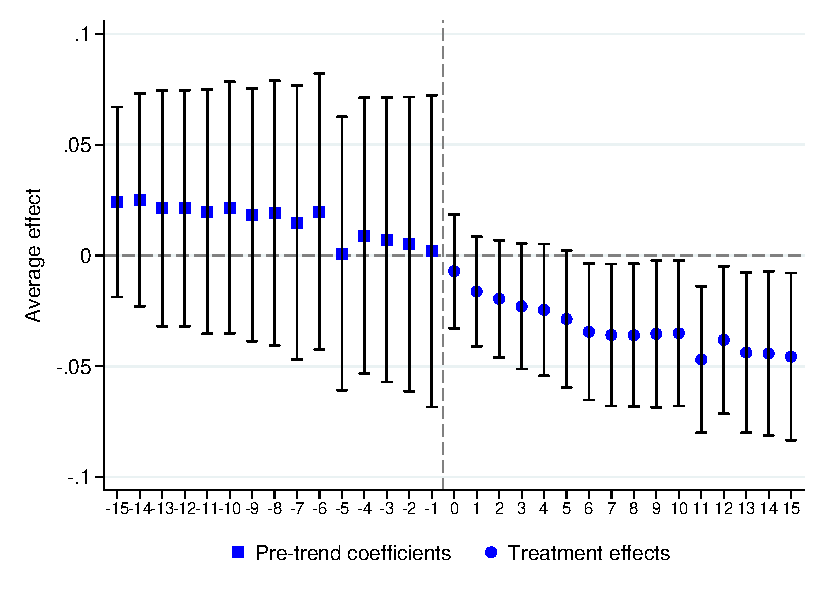
\includegraphics[scale=0.8]{FigureC2}\centering	
\end{figure}

\clearpage

\begin{figure}	
	\caption{FIGURE C3} 
		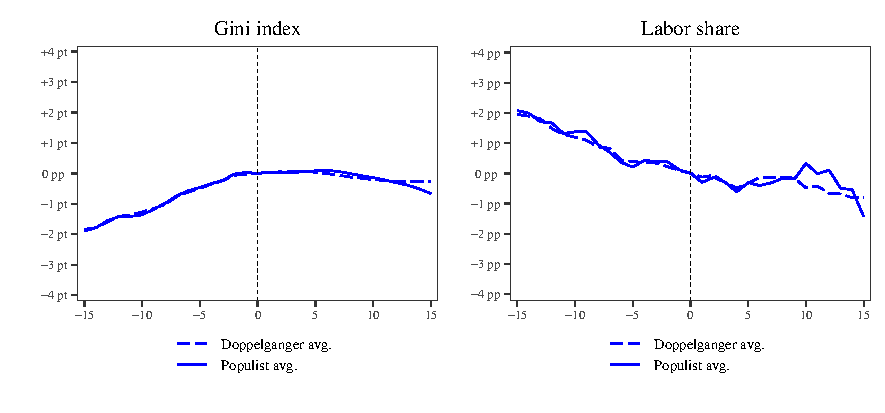
\includegraphics[scale=0.8]{FigureC3}\centering	
\end{figure}

\clearpage

\begin{figure}	
	\caption{FIGURE C4} 
		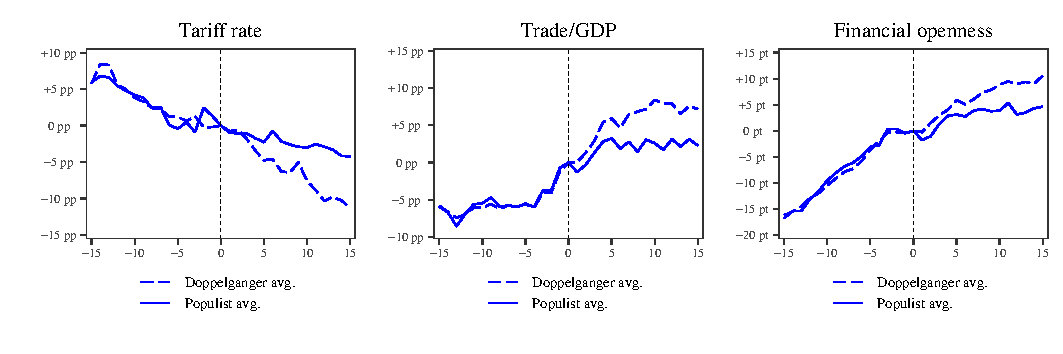
\includegraphics[scale=0.8]{FigureC4}\centering	
\end{figure}

\clearpage

\begin{figure}	
	\caption{FIGURE C5} 
		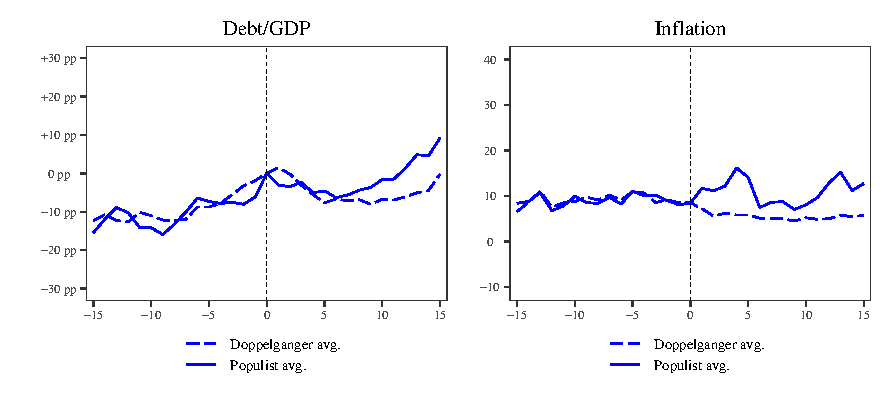
\includegraphics[scale=0.8]{FigureC5}\centering	
\end{figure}

\clearpage

\begin{figure}	
	\caption{FIGURE C6} 
		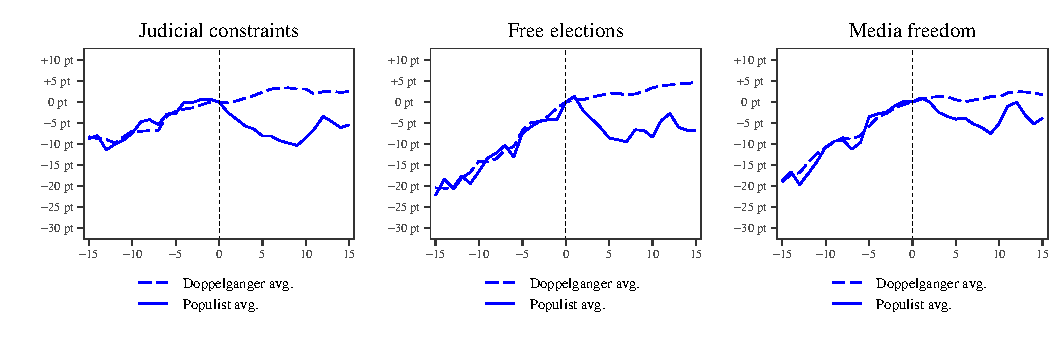
\includegraphics[scale=0.8]{FigureC6}\centering	
\end{figure}

\clearpage

\begin{figure}	
	\caption{FIGURE C7} 
		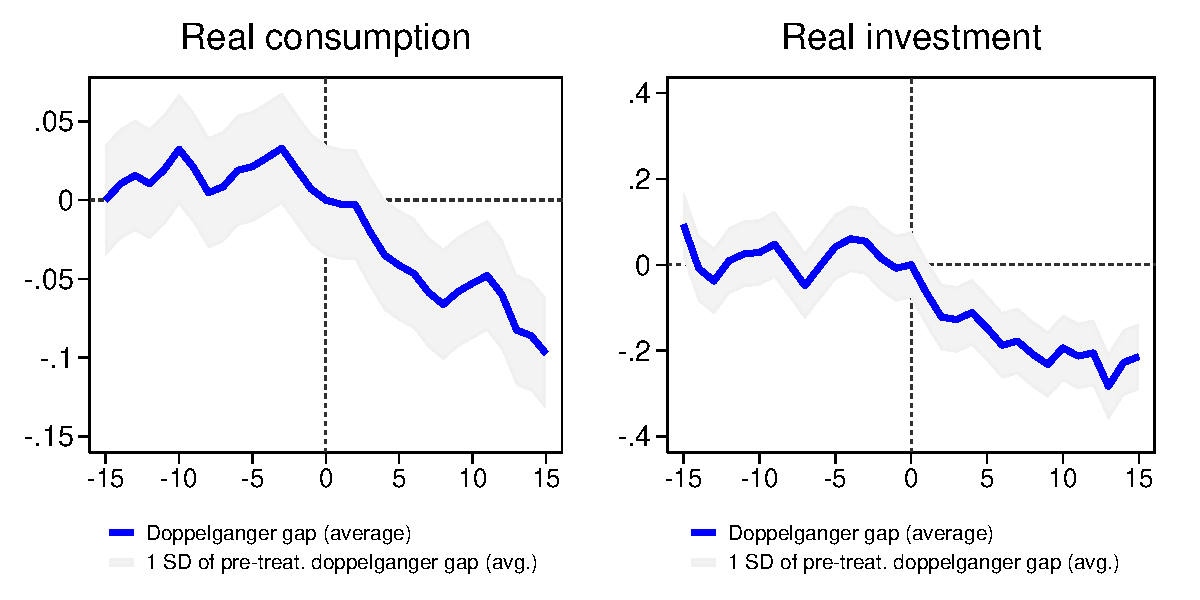
\includegraphics[scale=0.7]{FigureC7}\centering	
\end{figure}


\end{document}
